% SAHARA, IEEE conference version (6 pages). Numbers come from docs/evaluation_report.md and
% docs/name_call_eval.md (run models/logs/20261030-185320_a_real_s3). Build: tectonic -X compile sahara_ieee.tex
\documentclass[conference]{IEEEtran}
\usepackage{cite}
\usepackage{amsmath,amssymb,amsfonts}
\usepackage{graphicx}
\usepackage{textcomp}
\usepackage{xcolor}
\usepackage{booktabs}
\usepackage[hyphens]{url}
\usepackage{tikz}
\usetikzlibrary{arrows.meta,positioning,calc}
\newcommand{\INR}{Rs.~}

\begin{document}

\title{SAHARA: Real-Time On-Device Sound Event Detection and Alerting for Deaf and Hard-of-Hearing Users, with India-Specific Acoustic Adaptation}

\author{\IEEEauthorblockN{Mahi Mayani, Advika Mishra, Prachi Teotia, Raj Singh, Priti Rumao}
\IEEEauthorblockA{\textit{Department of Computer Engineering} \\
\textit{Mukesh Patel School of Technology Management \& Engineering (MPSTME)}\\
\textit{SVKM's NMIMS (Deemed-to-be University)}\\
Mumbai, India \\
priti.rumao@nmims.edu}}

\maketitle

\begin{abstract}
Deaf and hard-of-hearing (DHH) people miss safety-critical sounds such as smoke alarms and sirens, yet sound-recognition aids rarely report how often they alert falsely and are seldom tested outside Western homes. We present SAHARA, a fully on-device Android system that runs a frozen YAMNet encoder with a 296k-parameter classifier head for eight household sound classes and sends class-coded vibration alerts to the phone and to a proposed low-cost ESP32 wristband. Each class's threshold and temporal rule are tuned jointly against an explicit budget of false alarms per hour, with safety classes weighted three times. On held-out public data the system reaches 0.778 mAP at 3.5 false alarms per hour of continuous background audio, and the tuning cuts false alarms from 34.1 to 6.1 per hour on the same model. We also contribute SAHARA-IN, 329 sound clips and 107 name-call clips recorded in Mumbai homes and streets. Cross-validated mAP on them rises from 0.621 to 0.822 when recordings from the same sessions join training, but not when whole sessions are held out (0.600); a three-recording home calibration step instead raises the share of events alerted in unseen homes from 19\,\% to 35\,\%. A speech-embedding spotter tells users when their name is called and by whom.
\end{abstract}

\begin{IEEEkeywords}
assistive technology, deaf and hard of hearing, sound event detection, on-device machine learning, haptic feedback
\end{IEEEkeywords}

\section{Introduction}
More than 1.5 billion people live with some degree of hearing loss and over 430 million with disabling loss \cite{who2021}; in India an estimated 63 million people have significant auditory impairment \cite{nppcd}. For them, everyday sounds that carry safety or social information (a smoke alarm, a siren, a doorbell, a baby crying, someone calling their name) are inaudible unless converted to a visual or tactile signal. DHH users consistently rank alarms and safety sounds as the most important to be notified about and prefer glanceable, wearable and private notifications \cite{bragg2016,findlater2019,goodman2020}.

Deep audio embeddings trained on AudioSet \cite{gemmeke2017} have made sound recognition on phones and watches practical \cite{jain2020homesound,jain2020soundwatch,jain2022protosound,laput2018}. Three gaps remain. First, systems are evaluated with symmetric, threshold-free metrics, yet what users experience is a stream of alerts: a missed fire alarm can be fatal, and frequent false alerts lead users to ignore the aid \cite{jain2020homesound,huang2023}. Second, many prototypes send audio or features to a server, which is unacceptable for an always-listening device in the home. Third, public corpora come mostly from Western environments; Indian homes add pressure-cooker whistles, temple bells, hawkers and monsoon rain, and their doorbells are often melodic chimes.

SAHARA addresses these gaps with five contributions: (1) alert rules tuned against an explicit false-alarm budget; (2) fully on-device inference that never stores audio; (3) name-call alerts for any voice, naming enrolled callers; (4) SAHARA-IN, a field set from Indian homes, evaluated with a session-held-out protocol, and a home-calibration step; and (5) an open wristband design whose protocol and firmware are implemented and whose hardware is our next step.

\section{Related Work}
\textit{Sound awareness for DHH users.} Matthews et al. studied visualisations of non-speech sound \cite{matthews2006}, and Bragg et al. designed a personalisable mobile sound detector \cite{bragg2016}. In a survey of 201 DHH participants, Findlater et al. found strong interest in sound awareness on wearable and mobile devices \cite{findlater2019}, and Goodman et al. evaluated smartwatch sound feedback across contexts \cite{goodman2020}. Jain et al. deployed HomeSound in homes and found that false alerts quickly erode trust \cite{jain2020homesound}; SoundWatch moved recognition to a smartwatch and analysed accuracy, latency and battery trade-offs \cite{jain2020soundwatch}. Huang et al. ran a three-week field study of mobile sound recognition with DHH participants and reported that background noise, sound variability and confusable classes remain obstacles \cite{huang2023}. ProtoSound personalises recognition from a few examples with prototypical networks \cite{jain2022protosound,snell2017}, Goodman et al. studied user-driven personalisation \cite{goodman2021}, and UbiEar brought location-independent sound awareness to smartphones \cite{liu2017ubiear}. Earlier wearable prototypes also used smartwatches as the delivery device \cite{mielke2015}. These systems report accuracy on clips rather than alerts per hour of real audio, and were evaluated in North American or European homes.

\textit{Audio embeddings and detection.} VGGish \cite{hershey2017}, OpenL3 \cite{cramer2019}, PANNs \cite{kong2020}, the Audio Spectrogram Transformer \cite{gong2021} and YAMNet \cite{yamnet}, a MobileNetV1 \cite{howard2017} trained on AudioSet, provide transferable embeddings; data augmentation and weak labels are standard tools for small environmental-sound sets \cite{salamon2017,kumar2016}. Ubicoustics showed that such models transfer to real-world activity recognition \cite{laput2018}. We use YAMNet because it runs continuously on Android phones and exports to TensorFlow Lite \cite{jacob2018}. FSD50K \cite{fonseca2022}, AudioSet \cite{gemmeke2017}, ESC-50 \cite{piczak2015} and DESED \cite{turpault2019} are standard sources of domestic events; Mesaros et al. review detection metrics \cite{mesaros2016,mesaros2021}. Cost-sensitive learning is well established \cite{elkan2001}; we carry the cost asymmetry past the loss into the alert rule itself.

\textit{Keyword spotting and speaker recognition.} Speech embeddings pretrained for keyword spotting let a small head learn a new word from few examples \cite{lin2020}, as packaged by openWakeWord \cite{openwakeword}; GE2E training gives compact speaker embeddings for verification \cite{wan2018}.

\section{System Design}\label{sec:system}
\begin{figure*}[t]
\centering
\resizebox{\textwidth}{!}{%
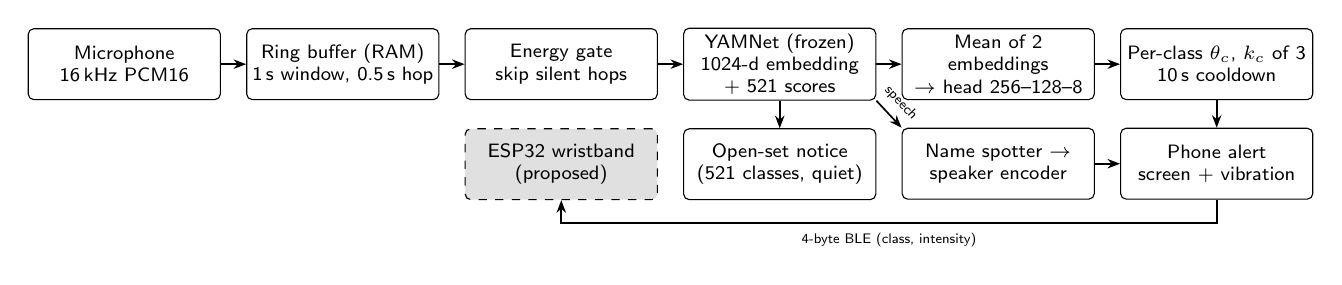
\begin{tikzpicture}[
  node distance=3.5mm and 3.2mm,
  box/.style={draw, rounded corners=2pt, align=center, font=\sffamily\scriptsize, text width=23mm, minimum height=9mm, inner sep=2pt, fill=white},
  arr/.style={-{Stealth[length=1.6mm]}, semithick}]
\node[box] (mic) {Microphone\\16\,kHz PCM16};
\node[box, right=of mic] (ring) {Ring buffer (RAM)\\1\,s window, 0.5\,s hop};
\node[box, right=of ring] (vad) {Energy gate\\skip silent hops};
\node[box, right=of vad] (yam) {YAMNet (frozen)\\1024-d embedding\\+ 521 scores};
\node[box, right=of yam] (head) {Mean of 2 embeddings\\$\rightarrow$ head 256--128--8};
\node[box, right=of head] (pol) {Per-class $\theta_c$, $k_c$ of 3\\10\,s cooldown};
\node[box, below=of yam] (other) {Open-set notice\\(521 classes, quiet)};
\node[box, below=of head] (name) {Name spotter $\rightarrow$\\speaker encoder};
\node[box, below=of pol] (alert) {Phone alert\\screen + vibration};
\node[box, left=of other, fill=black!12, dashed] (band) {ESP32 wristband\\(proposed)};
\draw[arr] (mic) -- (ring); \draw[arr] (ring) -- (vad); \draw[arr] (vad) -- (yam);
\draw[arr] (yam) -- (head); \draw[arr] (head) -- (pol); \draw[arr] (pol) -- (alert);
\draw[arr] (yam) -- (other); \draw[arr] (yam.south east) -- node[font=\sffamily\tiny, above, sloped]{speech} (name.north west);
\draw[arr] (name) -- (alert); \draw[arr] (alert.south) -- ++(0,-3mm) -| node[font=\sffamily\tiny, pos=0.25, below]{4-byte BLE (class, intensity)} (band.south);
\end{tikzpicture}}
\caption{SAHARA pipeline. Everything runs on the phone in an Android foreground service; only a class identifier and an intensity byte cross the Bluetooth link to the proposed wristband (dashed).}
\label{fig:arch}
\end{figure*}

Fig.~\ref{fig:arch} shows the pipeline. A native Kotlin foreground service captures 16\,kHz mono audio, so detection continues with the screen off. Samples enter a 1\,s RAM ring buffer that advances every 0.5\,s; a mean-square energy gate ($10^{-4}$) skips silent hops. Each remaining 0.975\,s patch is embedded by a frozen YAMNet into a 1024-dimensional vector, and the same pass yields YAMNet's 521 AudioSet scores. The mean of the two latest non-silent embeddings feeds a head (Dense 256 and 128 with ReLU and dropout, Dense 8 with sigmoid) of 296{,}328 parameters that scores smoke alarm, doorbell, siren, knocking, dog bark, baby cry, glass break and appliance beep independently. The training code computes exactly the same window vectors as the phone (tested to a maximum difference of 0.0), and 54 test clips replayed through the app's code raise the same alerts as the evaluation pipeline in 54 of 54 cases.

\textit{Privacy.} Audio exists only in the ring buffer and is overwritten every 0.5\,s; nothing is written to storage, the release build has no Internet permission, and enrolment keeps only embedding vectors.

\textit{Name calls and open-set notices.} When YAMNet's speech score is at least 0.2, pretrained speech embeddings \cite{lin2020,openwakeword} feed a logistic head that detects the user's name (``Aryan''). A GE2E speaker encoder \cite{wan2018} then compares the voice with family members enrolled once on the phone: at cosine similarity 0.70 or more the alert reads ``Raj is calling you'', otherwise ``Someone is calling you''. Sounds outside the eight classes that YAMNet recognises with score $\ge 0.35$ (e.g., a tap running) produce a quiet notice without vibration, so they never compete with safety alerts.

\textit{Haptics.} Each alert reaches the wristband as four bytes (version, command, class, intensity), and the phone and wristband play the same class-coded pattern (Fig.~\ref{fig:haptics}): the smoke alarm uses the ``temporal-three'' rhythm of evacuation alarms \cite{iso8201}, a siren swells, a doorbell is a strong-then-soft ``ding-dong'' and knocking is four taps. The wristband (ESP32, coin motor driven through a MOSFET, 500\,mAh cell, protected charger; about \INR 870) is designed and its firmware compiles; it has not yet been built or measured.

\begin{figure}[t]
\centering
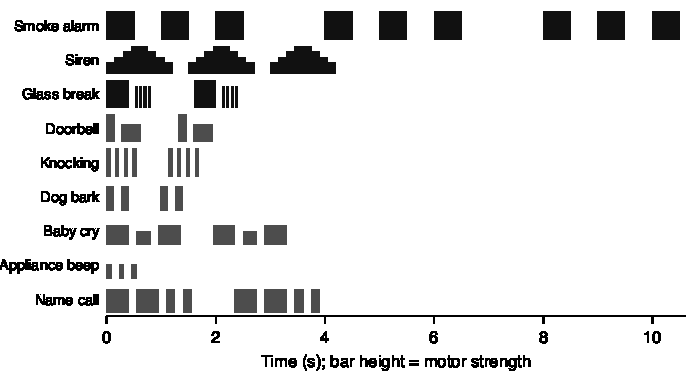
\includegraphics[width=\columnwidth]{figures/haptics.pdf}
\caption{Vibration patterns on one time scale, from the firmware; bar height is motor strength. Safety classes (top) use full strength.}
\label{fig:haptics}
\end{figure}

\section{Safety-Weighted Alerting}\label{sec:asym}
Smoke alarm, siren and glass break are safety-critical: their class weight is $w_c=3$, baby cry and appliance beep $1.5$, the rest $1$. The head is trained with a positive-weighted binary cross-entropy $\mathcal{L} = -\frac{1}{C}\sum_{c}[w_c y_c\log\hat{y}_c + (1-y_c)\log(1-\hat{y}_c)]$, so a missed positive costs up to three times a false positive \cite{elkan2001}. Sample weights balance classes and up-weight background windows eight times and SAHARA-IN clips ten times. Adam (learning rate $3\times10^{-4}$, batch 128) runs with early stopping.

\textit{Alert rule.} Class $c$ fires when its current window scores $s_{c,t}\ge\theta_c$, at least $k_c\in\{1,2,3\}$ of its last three windows are hits, and it has not fired within 10\,s. With a 1\,s window, 0.5\,s hop and two pooled embeddings, the worst-case decision latency for a sustained event is $W + 2H + (k_c-1)H + \tau = 2.0$--$3.0\,\mathrm{s}+\tau$, where $\tau$ is the inference time.

\textit{Tuning against a budget.} Instead of a fixed threshold we replay every validation clip through the exact rule and, for each candidate $(\theta_c,k_c)$, measure the detection rate $D_c$ (share of the class's clips that raise its alert) and the false-alarm rate $A_c$ (alerts per hour on validation audio without the class). We then solve
\begin{equation}
\max_{\{\theta_c,k_c\}}\ \sum_c w_c\,D_c(\theta_c,k_c)\quad\text{s.t.}\quad\sum_c A_c(\theta_c,k_c)\le B
\end{equation}
with a Lagrangian sweep and choose $B=4$ per hour (Fig.~\ref{fig:budget}). Run selection also uses only validation data: the best tuned score among runs trained on the current data, with safety-class precision of at least 0.70. Solving the same problem at $B\in\{1,2,4,8,16\}$ gives the app's five-step sensitivity setting, so every step has a measured trade-off.

\begin{figure}[t]
\centering
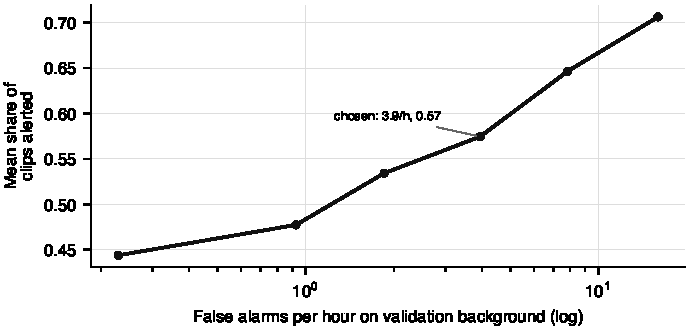
\includegraphics[width=\columnwidth]{figures/budget.pdf}
\caption{Mean share of validation clips alerted against the false-alarm budget (log scale), same model.}
\label{fig:budget}
\end{figure}

\section{Data and Protocol}\label{sec:data}
\textit{Public data.} Target clips come from FSD50K, AudioSet and ESC-50; background comes from 10{,}000 FSD50K clips without target-like labels, the 44 non-target ESC-50 categories and DESED soundscapes (Table~\ref{tab:data}). We verified every label identifier against the official vocabularies, which removed serious errors in an earlier build (e.g., AudioSet ``glass'' identifiers pointing to other classes and FSD50K's generic \textit{Alarm} mapped to appliance beep). Every class has at least 150 real clips and 20 in test. Splits are 70/15/15, grouped by upstream recording (YouTube or Freesound identifier) so one recording never appears in two splits. Each training target clip is also mixed onto three training-split backgrounds at $-5$ to 10\,dB SNR (6{,}834 mixtures); a separate set of 564 test mixtures is reported apart from real data.

\textit{Processing.} All audio is resampled to 16\,kHz mono. Each clip is cut into the same 1\,s windows the phone sees, embedded once by YAMNet and cached (22{,}521 clips). For weakly labelled clips, only the windows where YAMNet's own score for the class is highest are kept as positives; the rest of a target clip is dropped rather than used as background.

\textit{SAHARA-IN.} Four team members recorded 329 clips on their own phones in Mumbai homes and streets, in three uploads: 269 target clips (67 knocking, 59 appliance beep, 58 doorbell, 20 each of smoke alarm, siren and glass break, 14 baby cry, 11 dog bark) and 60 background clips (hawkers, a temple, a kitchen, television, monsoon rain, drawers and doors). About 40\,\% of each label is held out for test, and each upload is split on its own so new clips never move earlier ones. A further 107 clips (38 of the name ``Aryan'', 69 of similar names) serve the name-call model, evaluated leave-one-recorder-out. Because the recordings come from few sittings, we infer each clip's recording session (its recorder, or for unattributed uploads the phone's numbered file-name series) and also report cross-validation that holds out whole sessions.

\begin{table}[t]
\caption{Real clips per class (test clips in brackets); $^\dagger$ safety-critical. Background also includes 605 DESED clips.}
\label{tab:data}
\centering\footnotesize
\setlength{\tabcolsep}{3pt}
\resizebox{\columnwidth}{!}{%
\begin{tabular}{@{}lrrrrr@{}}
\toprule
Class & AudioSet & ESC-50 & FSD50K & SAHARA-IN & Total (test) \\
\midrule
Smoke alarm$^\dagger$ & 183 & -- & -- & 20 & 203 (35) \\
Doorbell & 92 & -- & 144 & 58 & 294 (57) \\
Siren$^\dagger$ & 34 & 40 & 132 & 20 & 226 (42) \\
Knocking & 97 & 40 & 373 & 67 & 577 (100) \\
Dog bark & 10 & 40 & 536 & 11 & 597 (94) \\
Baby cry & 106 & 40 & -- & 14 & 160 (30) \\
Glass break$^\dagger$ & 97 & 40 & 510 & 20 & 667 (105) \\
Appliance beep & 261 & 40 & 206 & 59 & 566 (101) \\
Background & -- & 1{,}760 & 10{,}000 & 60 & 12{,}425 (1{,}876) \\
\bottomrule
\end{tabular}}
\end{table}

\textit{Heterogeneous sources.} The sources differ in recording device, level, length and labelling (human-verified FSD50K, weak AudioSet clip labels, curated ESC-50, synthetic DESED soundscapes, phone recordings). We limit the resulting bias in four ways: every clip passes through the same resampling, windowing and YAMNet embedding as the phone; weak labels are reduced to the windows that contain the event; splits are grouped by source recording so no recording appears in two splits; and results are reported separately for public, Indian and synthetic test data rather than pooled. Table~\ref{tab:timeline} gives the order in which the data were collected and processed.

\begin{table}[t]
\caption{Data collection and processing timeline (2026).}
\label{tab:timeline}
\centering\footnotesize
\setlength{\tabcolsep}{3pt}
\begin{tabular}{@{}lp{6.3cm}@{}}
\toprule
When & Step \\
\midrule
Aug & Public data downloaded (FSD50K, AudioSet, ESC-50, DESED); manifest builder \\
Sep & SAHARA-IN first upload (team recordings, 16--17 Sep); synthetic mixing \\
Early Oct & Label identifiers audited and fixed; leak-free grouped splits; window-level YAMNet cache; budget-tuned alerting \\
29--30 Oct & SAHARA-IN uploads 2 and 3 (95 and 161 clips, incl.\ first smoke alarms, sirens, glass breaks); retraining; session-held-out evaluation; home calibration \\
\bottomrule
\end{tabular}
\end{table}

\textit{Metrics.} We report per-class AP over 0.5\,s windows, its mean (mAP), precision, recall and F1 at the tuned thresholds, the share of test clips that raise the correct alert under the deployed rule, and false alarms per hour with background audio played as one continuous stream. The test split was used once.

\section{Results}
\textit{Detection.} On the public test set the model reaches 0.778 mAP and a macro F1 of 0.670 (Table~\ref{tab:perclass}), and played as a stream through the deployed rule it raises 3.5 false alarms per hour on 3.4\,h of test background, mostly ``siren''. The safety classes are strongest: 22 of 27 smoke-alarm and 28 of 34 siren clips raise an alert. Knocking (AP 0.604) and appliance beep (0.567) are weakest; their brief, varied sounds limit the model rather than the rule (Fig.~\ref{fig:budget}). On the synthetic mixtures at $-5$ to 10\,dB, mAP falls to 0.666, so loud background remains the main challenge. Max-pooling instead of averaging the two embeddings, tried to keep brief sounds from being diluted, changed nothing (validation score 0.609 vs.\ 0.614 over five seeds).

\begin{table}[t]
\caption{Public test set per class at the deployed rule: threshold $\theta_c$, windows $k_c$ of 3, window AP and F1, and clips alerted.}
\label{tab:perclass}
\centering\footnotesize
\setlength{\tabcolsep}{4pt}
\begin{tabular}{@{}lrrrrr@{}}
\toprule
Class & $\theta_c$ & $k_c$ & AP & F1 & Clips alerted \\
\midrule
Smoke alarm$^\dagger$ & 0.81 & 2 & 0.916 & 0.858 & 22/27 \\
Doorbell & 0.995 & 1 & 0.711 & 0.432 & 13/35 \\
Siren$^\dagger$ & 0.91 & 1 & 0.875 & 0.817 & 28/34 \\
Knocking & 0.95 & 1 & 0.604 & 0.410 & 21/73 \\
Dog bark & 0.98 & 1 & 0.908 & 0.847 & 67/90 \\
Baby cry & 0.99 & 2 & 0.817 & 0.712 & 17/25 \\
Glass break$^\dagger$ & 0.93 & 1 & 0.827 & 0.790 & 56/97 \\
Appliance beep & 0.90 & 3 & 0.567 & 0.496 & 17/78 \\
\midrule
Mean & & & 0.778 & 0.670 & 0.56 \\
\bottomrule
\end{tabular}
\end{table}

\textit{What the tuning buys.} Replaying all 2{,}435 real test clips (4.6\,h) through three rules on the same model (Table~\ref{tab:ablation}; false alarms here count alerts for a class on any audio without it, so they exceed the background-only figure), a fixed threshold of 0.5 with 2-of-3 smoothing gives 34.1 false alarms per hour, more than one every two minutes. Budget tuning brings this to 6.1 while still alerting on 54\,\% of clips and 69\,\% of safety clips. The sensitivity steps span 47\,\% of clips at 2.5 false alarms per hour to 67\,\% at 20.6.

\begin{table}[t]
\caption{Same model, three alert rules, all real test audio.}
\label{tab:ablation}
\centering\footnotesize
\setlength{\tabcolsep}{3pt}
\begin{tabular}{@{}lrrr@{}}
\toprule
Alert rule & Clips & Safety & FA/h \\
\midrule
$\theta=0.5$, 1 window & 0.766 & 0.838 & 49.1 \\
$\theta=0.5$, 1 (safety) or 2 of 3 windows & 0.688 & 0.838 & 34.1 \\
Tuned $(\theta_c,k_c)$, $B=4$/h (SAHARA) & 0.538 & 0.692 & 6.1 \\
\bottomrule
\end{tabular}
\end{table}

\textit{Indian conditions.} In five-fold cross-validation over the 329 SAHARA-IN clips with random folds, adding them to training raises mAP from 0.621 to 0.822 and the clips alerted from 45 to 100 of 269; smoke alarm AP rises from 0.385 to 0.801 and doorbell from 0.521 to 0.824. Holding out whole recording sessions instead, the gain disappears (0.621 vs.\ 0.600), although doorbells still improve (0.521 to 0.691). The recordings therefore teach the model a particular home's sounds far better than Indian sounds in general, and the held-out test split (0.831 mAP; 0.698 for a model trained before the latest upload) overstates transfer to a new home.

\textit{Home calibration.} This motivates a calibration step: the user records a sound three times where it happens; the app sets that class's threshold 0.5 log-odds below the weakest recording's firing level, never below its threshold at the 16-per-hour sensitivity step, and an optional recording of ordinary home sound raises it again if needed. On session-held-out models (three clips of an unseen session as calibration, the rest as events, 20 draws), the share of events alerted across 17 session--class pairs rises from 19\,\% to 35\,\%, for about one extra false alarm per hour per calibrated class. Doorbells gain most (e.g., 20\,\% to 83\,\%); knocking and glass break do not, because their scores stay below even the most permissive tested threshold.

\textit{Name calls.} Leaving one recorder out, the name spotter separates calls of ``Aryan'' from background scenes with ROC AUC 0.872 (equal error rate 19\,\%) and from similar names such as Arya and Aryanshi with AUC 0.743 (32\,\%). Caller identification names the right person in 29 of 38 calls; with a caller not enrolled, 82\,\% of their calls read ``Someone''.

\textit{On-device cost.} On a Samsung Galaxy S24 (Android 16), inference takes 20--29\,ms per window with the screen on and 47--49\,ms with it off, the models occupy 15.0\,MB (YAMNet), 1.2\,MB (head) and 8.1\,MB (name call), the release APK is 45.8\,MB, and memory use is 128.9\,MB. In a speaker test the phone alerted 1.0--2.5\,s after sound onset, within the latency bound above.

\section{Discussion and Limitations}
At 4 false alarms per hour the model alerts on about 58\,\% of validation events, and quadrupling the budget raises this only to 71\,\%, so brief sounds need a stronger model (e.g., fine-tuning YAMNet's last layers) or more data, not a looser rule. SAHARA-IN is small, with 20 clips per safety class, and comes from few sessions, so claims about unseen Indian homes need many more households. The name spotter is trained for one name and confuses similar names about a third of the time; its speech models are licensed for non-commercial use. We have not yet built the wristband, measured battery drain over a day, or run a study with DHH participants; a field deployment in Mumbai measuring missed events, alert fatigue and recognition of the haptic patterns is planned \cite{findlater2019,huang2023}.

\section{Conclusion}
SAHARA shows that sound awareness for DHH users can run entirely on a phone, retain no audio and be tuned for the number that decides whether users keep it on: false alarms per hour. Tuning each class's threshold and temporal rule against an explicit budget cut false alarms more than five-fold on the same model. Field recordings from Indian homes taught the model those homes' sounds but not yet unseen ones, and a three-recording calibration step recovers much of that gap. A separate speech path tells users when they are called and by whom. Code, alert tuning, Bluetooth protocol, firmware and the SAHARA-IN protocol are released.

\begin{thebibliography}{00}
\bibitem{who2021} World Health Organization, \textit{World Report on Hearing}. Geneva: WHO, 2021.
\bibitem{nppcd} Directorate General of Health Services, Ministry of Health \& Family Welfare, Government of India, ``National Programme for Prevention and Control of Deafness (NPPCD).'' [Online]. Available: \url{https://dghs.mohfw.gov.in}
\bibitem{bragg2016} D. Bragg, N. Huynh, and R. E. Ladner, ``A personalizable mobile sound detector app design for deaf and hard-of-hearing users,'' in \textit{Proc. ACM SIGACCESS Conf. Computers and Accessibility (ASSETS)}, 2016, pp. 3--13.
\bibitem{findlater2019} L. Findlater, B. Chinh, D. Jain, J. Froehlich, R. Kushalnagar, and A. C. Lin, ``Deaf and hard-of-hearing individuals' preferences for wearable and mobile sound awareness technologies,'' in \textit{Proc. CHI Conf. Human Factors in Computing Systems}, 2019.
\bibitem{goodman2020} S. M. Goodman, P. Kirchner, R. Guttman, D. Jain, J. Froehlich, and L. Findlater, ``Evaluating smartwatch-based sound feedback for deaf and hard-of-hearing users across contexts,'' in \textit{Proc. CHI Conf. Human Factors in Computing Systems}, 2020.
\bibitem{gemmeke2017} J. F. Gemmeke \textit{et al.}, ``Audio Set: An ontology and human-labeled dataset for audio events,'' in \textit{Proc. IEEE ICASSP}, 2017, pp. 776--780.
\bibitem{jain2020homesound} D. Jain \textit{et al.}, ``HomeSound: An iterative field deployment of an in-home sound awareness system for deaf or hard of hearing users,'' in \textit{Proc. CHI Conf. Human Factors in Computing Systems}, 2020.
\bibitem{jain2020soundwatch} D. Jain, H. Ngo, P. Patel, S. Goodman, L. Findlater, and J. Froehlich, ``SoundWatch: Exploring smartwatch-based deep learning approaches to support sound awareness for deaf and hard of hearing users,'' in \textit{Proc. ACM ASSETS}, 2020.
\bibitem{jain2022protosound} D. Jain \textit{et al.}, ``ProtoSound: A personalized and scalable sound recognition system for deaf and hard-of-hearing users,'' in \textit{Proc. CHI Conf. Human Factors in Computing Systems}, 2022.
\bibitem{laput2018} G. Laput, K. Ahuja, M. Goel, and C. Harrison, ``Ubicoustics: Plug-and-play acoustic activity recognition,'' in \textit{Proc. ACM UIST}, 2018.
\bibitem{huang2023} J. Z. Huang, H. Chhabria, and D. Jain, ```Not there yet': Feasibility and challenges of mobile sound recognition to support deaf and hard-of-hearing people,'' in \textit{Proc. ACM ASSETS}, 2023, pp. 1--14.
\bibitem{matthews2006} T. Matthews, J. Fong, F. W.-L. Ho-Ching, and J. Mankoff, ``Evaluating non-speech sound visualizations for the deaf,'' \textit{Behav. Inf. Technol.}, vol. 25, no. 4, pp. 333--351, 2006.
\bibitem{snell2017} J. Snell, K. Swersky, and R. Zemel, ``Prototypical networks for few-shot learning,'' in \textit{Proc. NeurIPS}, vol. 30, 2017.
\bibitem{goodman2021} S. M. Goodman \textit{et al.}, ``Toward user-driven sound recognizer personalization with people who are d/Deaf or hard of hearing,'' \textit{Proc. ACM Interact. Mob. Wearable Ubiquitous Technol.}, vol. 5, no. 2, 2021.
\bibitem{liu2017ubiear} S. Liu, Z. Zhou, J. Du, L. Shangguan, J. Han, and X. Wang, ``UbiEar: Bringing location-independent sound awareness to the hard-of-hearing people with smartphones,'' \textit{Proc. ACM Interact. Mob. Wearable Ubiquitous Technol.}, vol. 1, no. 2, 2017.
\bibitem{mielke2015} M. Mielke and R. Br\"uck, ``A pilot study about the smartwatch as assistive device for deaf people,'' in \textit{Proc. ACM ASSETS}, 2015, pp. 301--302.
\bibitem{hershey2017} S. Hershey \textit{et al.}, ``CNN architectures for large-scale audio classification,'' in \textit{Proc. IEEE ICASSP}, 2017, pp. 131--135.
\bibitem{cramer2019} J. Cramer, H.-H. Wu, J. Salamon, and J. P. Bello, ``Look, listen, and learn more: Design choices for deep audio embeddings,'' in \textit{Proc. IEEE ICASSP}, 2019, pp. 3852--3856.
\bibitem{kong2020} Q. Kong, Y. Cao, T. Iqbal, Y. Wang, W. Wang, and M. D. Plumbley, ``PANNs: Large-scale pretrained audio neural networks for audio pattern recognition,'' \textit{IEEE/ACM Trans. Audio, Speech, Lang. Process.}, vol. 28, pp. 2880--2894, 2020.
\bibitem{gong2021} Y. Gong, Y.-A. Chung, and J. Glass, ``AST: Audio spectrogram transformer,'' in \textit{Proc. Interspeech}, 2021, pp. 571--575.
\bibitem{yamnet} M. Plakal and D. Ellis, ``YAMNet,'' TensorFlow Model Garden, 2020. [Online]. Available: \url{https://github.com/tensorflow/models/tree/master/research/audioset/yamnet}
\bibitem{howard2017} A. G. Howard \textit{et al.}, ``MobileNets: Efficient convolutional neural networks for mobile vision applications,'' arXiv:1704.04861, 2017.
\bibitem{salamon2017} J. Salamon and J. P. Bello, ``Deep convolutional neural networks and data augmentation for environmental sound classification,'' \textit{IEEE Signal Process. Lett.}, vol. 24, no. 3, pp. 279--283, 2017.
\bibitem{kumar2016} A. Kumar and B. Raj, ``Audio event detection using weakly labeled data,'' in \textit{Proc. ACM Multimedia}, 2016, pp. 1038--1047.
\bibitem{jacob2018} B. Jacob \textit{et al.}, ``Quantization and training of neural networks for efficient integer-arithmetic-only inference,'' in \textit{Proc. IEEE CVPR}, 2018, pp. 2704--2713.
\bibitem{fonseca2022} E. Fonseca, X. Favory, J. Pons, F. Font, and X. Serra, ``FSD50K: An open dataset of human-labeled sound events,'' \textit{IEEE/ACM Trans. Audio, Speech, Lang. Process.}, vol. 30, pp. 829--852, 2022.
\bibitem{piczak2015} K. J. Piczak, ``ESC: Dataset for environmental sound classification,'' in \textit{Proc. ACM Multimedia}, 2015, pp. 1015--1018.
\bibitem{turpault2019} N. Turpault, R. Serizel, A. Parag Shah, and J. Salamon, ``Sound event detection in domestic environments with weakly labeled data and soundscape synthesis,'' in \textit{Proc. Detection and Classification of Acoustic Scenes and Events Workshop (DCASE)}, 2019, pp. 253--257.
\bibitem{mesaros2016} A. Mesaros, T. Heittola, and T. Virtanen, ``Metrics for polyphonic sound event detection,'' \textit{Applied Sciences}, vol. 6, no. 6, p. 162, 2016.
\bibitem{mesaros2021} A. Mesaros, T. Heittola, T. Virtanen, and M. D. Plumbley, ``Sound event detection: A tutorial,'' \textit{IEEE Signal Process. Mag.}, vol. 38, no. 5, pp. 67--83, 2021.
\bibitem{elkan2001} C. Elkan, ``The foundations of cost-sensitive learning,'' in \textit{Proc. IJCAI}, 2001, pp. 973--978.
\bibitem{lin2020} J. Lin, K. Kilgour, D. Roblek, and M. Sharifi, ``Training keyword spotters with limited and synthesized speech data,'' in \textit{Proc. IEEE ICASSP}, 2020, pp. 7474--7478.
\bibitem{openwakeword} D. Scripka, ``openWakeWord,'' GitHub, 2023. [Online]. Available: \url{https://github.com/dscripka/openWakeWord}
\bibitem{wan2018} L. Wan, Q. Wang, A. Papir, and I. Lopez Moreno, ``Generalized end-to-end loss for speaker verification,'' in \textit{Proc. IEEE ICASSP}, 2018, pp. 4879--4883.
\bibitem{iso8201} ISO 8201:2017, \textit{Alarm systems---Audible emergency evacuation signal---Requirements}. Geneva: ISO, 2017.
\end{thebibliography}

\end{document}
